\documentclass{../paper}

\newcommand{\fig}[1]{Fig.~#1}
\newcommand{\tab}[1]{Table~#1}
\newcommand{\eq}[1]{Eq.~#1}
\newcommand{\eqs}[2]{Eqs.~#1--#2}

\begin{document}

\title{Investigating Crystal Structures with X-Ray Diffraction}

\author{Iago B.~Mendes\,\orcidlink{0009-0007-9845-8448}}
\email{ibrazmen@oberlin.edu}
\affiliation{Department of Physics and Astronomy, Oberlin College, Oberlin, Ohio 44074, USA}

\date{\today}

\begin{abstract}
  In this experiment, we used X-ray diffraction to study the crystal structures of polycrystalline silicon, single-crystal silicon, and a high-temperature superconductor. For the polycrystalline sample, we identified several peaks and determined the lattice parameter to be $a = 5.4318(3)$ \AA{}, after correcting for a sample offset. In the single-crystal measurements, we determined that one sample was cut along the (400) symmetry plane and confirmed the absence of peaks in a sample with a (510) cut. Finally, we compared two superconductor samples prepared under different conditions and found that their diffraction patterns were nearly identical. To improve accuracy in our analysis, we modeled each peak as a $K\alpha$ doublet using a sum of Voigt profiles. These results demonstrate the precision of X-ray diffraction in characterizing crystal structures.
\end{abstract}

\maketitle

\section{Introduction}

X-rays were discovered in 1895 by Wilhelm Röntgen, who observed a new form of radiation capable of penetrating opaque materials and exposing photographic plates \cite{Roentgen1896}. Their wave nature was confirmed in 1912, when Max von Laue demonstrated that crystals could diffract X-rays, revealing the periodic atomic structure of solids \cite{Laue1912}. This discovery marked the beginning of X-ray crystallography and earned von Laue the Nobel Prize in Physics in 1914. One year later, William Henry Bragg and William Lawrence Bragg developed a simple model for interpreting X-ray diffraction patterns \cite{Bragg1913}. Their formulation, known as Bragg's law, related the diffraction angle to the spacing between atomic planes, providing a practical method for determining crystal structures and earning them the Nobel Prize in Physics in 1915.

Since then, X-ray diffraction has become one of the most powerful tools for investigating the atomic-scale structure of matter. Its continued relevance comes from its ability to probe internal structure without destroying the sample, making it indispensable in both research and industry \cite{Cullity}. Improvements in instrumentation and technique have dramatically increased the accuracy and sensitivity of diffraction experiments, enabling the resolution of fine spectral features such as the closely spaced $K\alpha_1$ and $K\alpha_2$ lines that were previously indistinguishable \cite{Cullity}. This level of detail allows for more reliable determination of lattice parameters and deeper insight into material behavior.

In this experiment, we use X-ray diffraction to investigate the crystal structure of different samples. In Section~\ref{sec:theory}, we review Bragg's law and discuss how diffraction patterns depend on crystal symmetry and atomic structure. Section~\ref{sec:methods} describes how we collect and analyze our data. In Section~\ref{sec:results}, we present our measurements and discuss the structural information obtained from each sample. Finally, we summarize our work in Section~\ref{sec:conclusion}.

\section{Theory}\label{sec:theory}

X-ray diffraction is a powerful technique for probing the atomic-scale structure of crystalline materials. When an incident beam of X-rays interacts with the periodic arrangement of atoms in a crystal, constructive interference occurs at specific angles, producing sharp diffraction peaks. This process is illustrated in \fig{\ref{fig:angles}}.

\begin{figure}
  \centering
  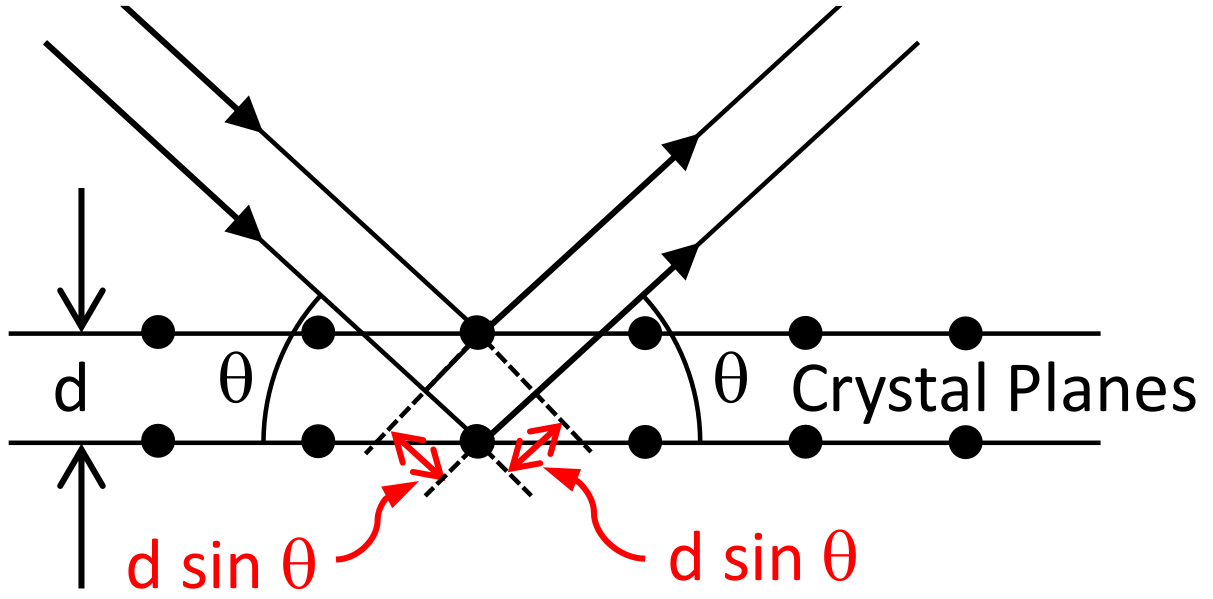
\includegraphics[width=0.6\columnwidth]{assets/bragg-scattering.png}
  \caption{Schematic representation of Bragg scattering. This figure is reproduced from \cite{LabManual}.}
  \label{fig:angles}
\end{figure}

The condition for constructive interference is given by Bragg's law:
\begin{equation} \label{eq:bragg}
  \lambda = 2 d \sin\theta
\end{equation}
\cite{Cullity}, where $\lambda$ is the wavelength of the incident X-rays, $d$ is the spacing between adjacent crystal planes, and $\theta$ is the angle of incidence. The wavelength is fixed by the choice of X-ray source, and the detector is rotated to scan over a range of angles $\theta$.

The location of each diffraction peak is determined by the geometry of the crystal lattice, while the relative intensity of each peak depends on the electron densities of the atoms in the material. Atoms with more electrons scatter X-rays more strongly, so peaks are more intense when they come from planes that contain heavier elements or higher concentrations of atoms. The specific arrangement of atoms also matters, since waves scattered from different atoms can interfere constructively or destructively depending on their positions.

For a crystal with cubic symmetry, the interplanar spacing $d$ associated with the Miller indices $(hkl)$ is given by:
\begin{equation} \label{eq:d-spacing}
  d_{hkl} = \frac{a}{\sqrt{h^2 + k^2 + l^2}}
\end{equation}
\cite{Cullity}, where $a$ is the lattice parameter. By measuring the diffraction angles associated with different peaks and applying Bragg's law, one can extract structural information such as the lattice constant $a$ and the orientation of single crystals.

If a material adopts a crystal structure with lower symmetry (such as tetragonal instead of cubic), we expect it to produce more diffraction peaks. This is because lower symmetry allows for more distinct sets of lattice planes, which increases the number of angles that satisfy \eq{\ref{eq:bragg}}. Moreover, changing the X-ray source alters the wavelength $\lambda$ and thus shifts the angular positions of all peaks according to \eq{\ref{eq:bragg}}.

\section{Methods}\label{sec:methods}

The following discussion is based on \cite{Laing}. X-rays in our diffractometer are produced when high-energy electrons strike a solid metal target. In our case, electrons are accelerated by a high-voltage potential and directed toward a copper anode. As the electrons collide with the target, their kinetic energy is converted into electromagnetic radiation. The resulting emission consists of two parts (see \fig{\ref{fig:x-rays}}): a black-body radiation background and sharp peaks known as characteristic lines. These characteristic lines are labeled $K\alpha$ and $K\beta$.

\begin{figure}
  \centering
  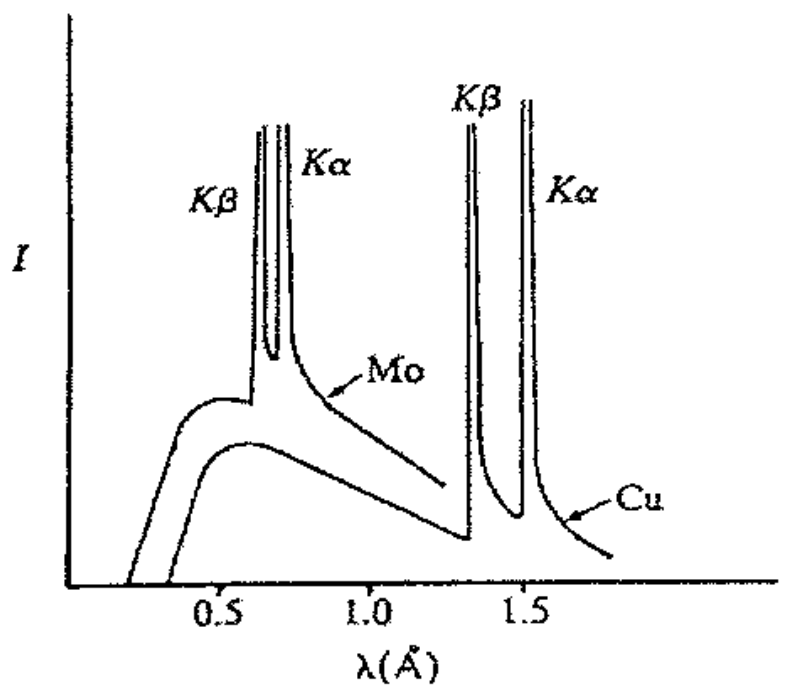
\includegraphics[width=0.6\columnwidth]{assets/Xray-source.png}
  \caption{Generation of X-rays for two sources: molybdenum (Mo) and copper (Cu). This figure is reproduced from \cite{Laing}.}
  \label{fig:x-rays}
\end{figure}

We used a Rigaku Ultima IV X-ray diffractometer, which is equipped with a copper anode. In our experiment, we want to use only the $K\alpha$ line. To isolate this specific wavelength, a graphite monochromator is used to filter out other components of the spectrum, such as the $K\beta$ line \cite{LabManual}. This allows us to produce a nearly monochromatic beam, which improves the precision of diffraction measurements by ensuring that the wavelength $\lambda$ in Bragg's law remains fixed throughout the scan. The intensity of scattered X-rays is measured by a detector mounted on a rotating arm that moves along with the X-ray source, which is why our data is presented as a function of $2\theta$.

Due to spin-coupling effects, the $K\alpha$ line consists of two closely spaced lines, $K\alpha_1$ and $K\alpha_2$, known as the $K\alpha$ doublet \cite{Cullity}. Their wavelengths are 1.54051~\AA{} and 1.54433~\AA{}, respectively \cite{Cullity}. The $K\alpha_1$ line is more intense, typically twice as strong as $K\alpha_2$, but both contribute to the measured diffraction pattern. At low angles, the difference in wavelength is small enough that the doublet appears as a single broadened peak. However, at higher angles, the two components become more distinguishable, leading to a visible splitting. To obtain accurate peak positions, it is important to correct for the presence of the doublet in the data analysis.

To analyze our X-ray diffraction data, we first used {\tt SciPy}'s {\tt find\_peaks} procedure \cite{SciPy} to identify approximate peak positions based on intensity and separation thresholds. Each identified peak was then modeled as a superposition of two Voigt profiles, corresponding to the $K\alpha_1$ and $K\alpha_2$ components of the copper X-ray emission. We fixed their angular separation based on their relative wavelengths and enforced the expected 2:1 intensity ratio. The fitting was performed using {\tt LMFIT}'s {\tt VoigtModel} class \cite{LMFIT}, which allows us to combine and constrain multiple peak models at once. By including both components in the fit, we account for the asymmetry introduced by the $K\alpha$ doublet and obtain more accurate estimates for the peak centers.

\section{Results}\label{sec:results}

We used X-ray diffraction to analyze three types of crystal structures, each with a specific goal. First, we measured a sample of polycrystalline silicon in order to determine its lattice parameter. Then, we measured two samples of single-crystal silicon: one with a “standard” cut, which we aimed to identify, and another with a (510) cut to confirm its orientation. Finally, we measured two samples of a superconductor to compare whether different preparation conditions affected their crystal structure.

\subsection{Polycrystalline silicon}

We began by measuring a sample of polycrystalline silicon to determine its lattice parameter. The resulting data and fits are shown in \fig{\ref{fig:peaks-poly}}. The double-peak feature of the first peak was not resolved in the full scan (\fig{\ref{fig:peaks-poly-b}}), so we performed a higher-resolution scan of that region (\fig{\ref{fig:peaks-poly-a}}). By comparing to literature values of silicon peaks \cite{Si}, we can identify the Miller indices (hkl) of each peak in \fig{\ref{fig:peaks-poly-b}} respectively as follows: (111), (220), (311), (400), (331), (422), (511). Using this peak identification, we can calculate the lattice parameter $a$ of the sample using \eqs{\eqref{eq:bragg}}{\eqref{eq:d-spacing}}. The results for each peak are shown in \tab{\ref{tab:lattice-parameter}}. Taking the average and standard deviation of these values, we find
\begin{equation}
  a = 5.428(1) \text{ \AA}.
\end{equation}
This result is three standard deviations away from the literature value \cite{Si}, $5.431$ \AA.

\begin{figure}
  \centering
  \begin{subfigure}{\columnwidth}
    \centering
    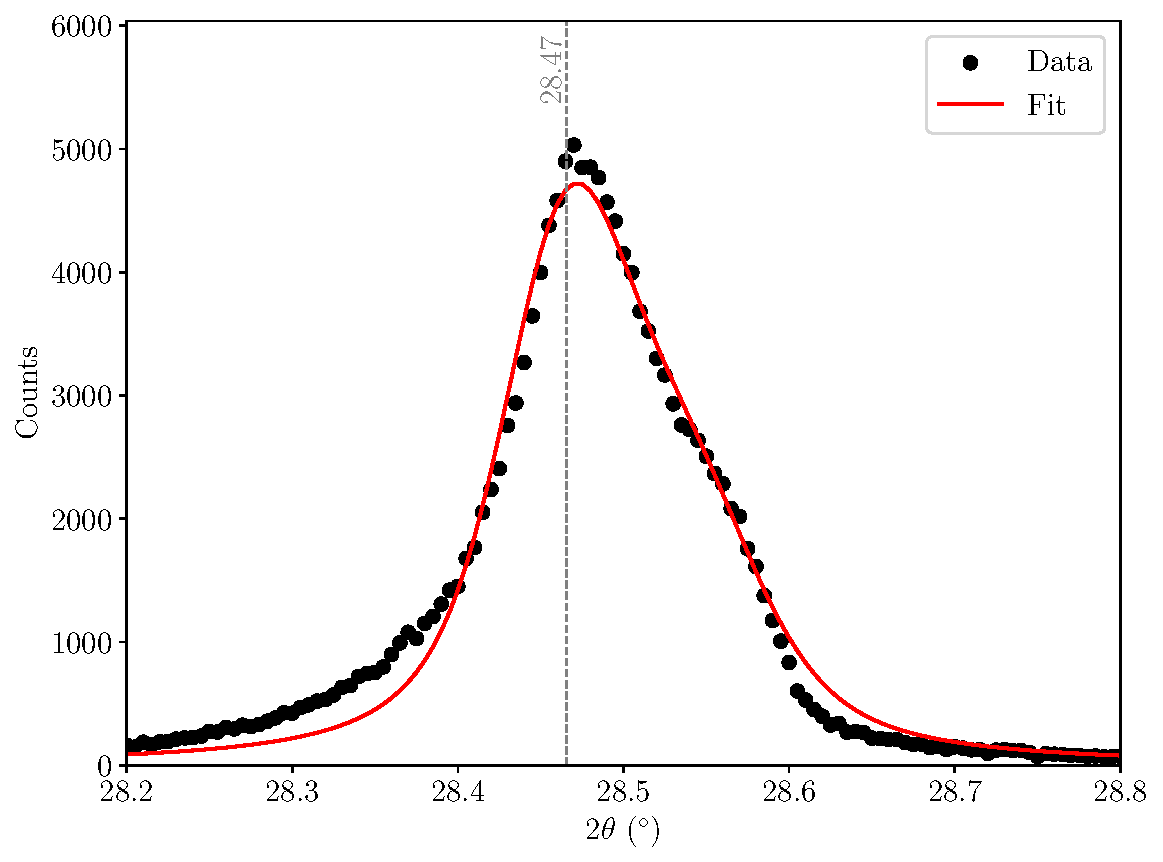
\includegraphics[width=\textwidth]{analysis/peaks-Si_polycrystalline-1st_peak.pdf}
    \caption{}
    \label{fig:peaks-poly-a}
  \end{subfigure}

  \begin{subfigure}{\columnwidth}
    \centering
    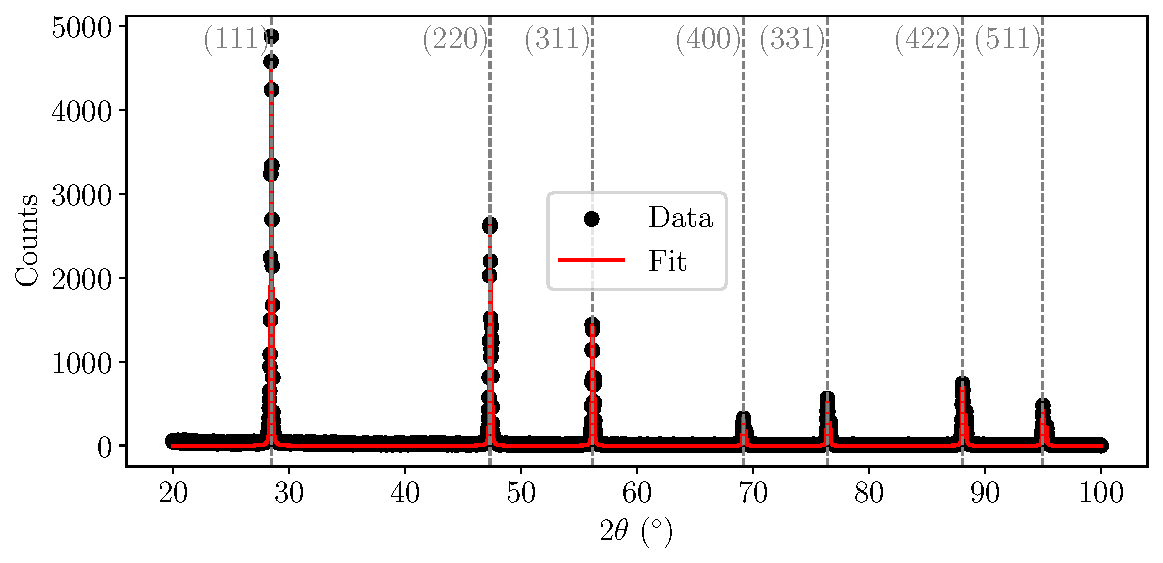
\includegraphics[width=\textwidth]{analysis/peaks-Si_polycrystalline.pdf}
    \caption{}
    \label{fig:peaks-poly-b}
  \end{subfigure}

  \caption{X-ray diffraction of polycrystalline silicon. (a) The first peak was scanned with higher precision to resolve the double peak feature. (b) The full scan of the sample.}
  \label{fig:peaks-poly}
\end{figure}

\begin{table}
  \centering
  \begin{tabular}{cccccc}
    $h$ & $k$ & $l$ & $2\theta$ (°) & $d$ (\AA) & $a$ (\AA) \\
    \hline
    1 & 1 & 1 & 28.464(5) & 3.133 & 5.427 \\
    2 & 2 & 0 & 47.33(2) & 1.919 & 5.428 \\
    3 & 1 & 1 & 56.15(2) & 1.637 & 5.428 \\
    4 & 0 & 0 & 69.16(2) & 1.357 & 5.429 \\
    3 & 3 & 1 & 76.41(2) & 1.245 & 5.429 \\
    4 & 2 & 2 & 88.06(2) & 1.108 & 5.429 \\
    5 & 1 & 1 & 94.99(2) & 1.045 & 5.429 \\
    \hline
  \end{tabular}
  \caption{Silicon lattice parameters for each peak in polycrystalline sample.}
  \label{tab:lattice-parameter}
\end{table}

Note the systematic trend in \tab{\ref{tab:lattice-parameter}}: the calculated values of $a$ increase with increasing $2\theta$. This is indicative that the sample had a vertical offset, which can be corrected. Differentiating \eqs{\ref{eq:bragg}}{\ref{eq:d-spacing}}, we find that a systematic error $\Delta\theta$ leads to an error in $a$ given by
\begin{equation}\label{eq:delta-a}
  \frac{\Delta a}{a} = - \cot\theta \Delta\theta
\end{equation}
\cite{Cullity}. If the sample has a height offset $\Delta h$, this will lead to a systematic error in $\theta$ given by
\begin{equation}\label{eq:delta-theta}
  \Delta\theta = - \frac{\Delta h}{R} \sin\theta \cos\theta
\end{equation}
\cite{Cullity}, where $R$ is the distance between the sample and the detector ($R = 285$ mm in our equipment).

Combining \eqs{\ref{eq:delta-a}}{\ref{eq:delta-theta}}, we can create a model for our measured lattice parameters:
\begin{equation}\label{eq:model}
  a = \frac{A}{1 - \frac{\Delta h}{R} \cos^2\theta},
\end{equation}
where $A$ is a constant. Using {\tt SciPy}'s {\tt curve\_fit} procedure \cite{SciPy}, we can fit \eq{\ref{eq:model}} to the data in \tab{\ref{tab:lattice-parameter}}. The resulting fit is shown in \fig{\ref{fig:fit-poly}}. The fit gives
\begin{align}
  A &= 5.4318(5) \text{ \AA}, \\
  \Delta h &= -0.26(4) \text{ mm},
\end{align}
which indicates that the sample was lower than the detector center. With this fit, we can find corrected lattice parameters, which are shown in the right panel of \fig{\ref{fig:fit-poly}}. Taking the average and standard deviation of these values, we find
\begin{equation}
  a = 5.4318(3) \text{ \AA},
\end{equation}
which agrees well with the literature value \cite{Si}.

\begin{figure}
  \centering
  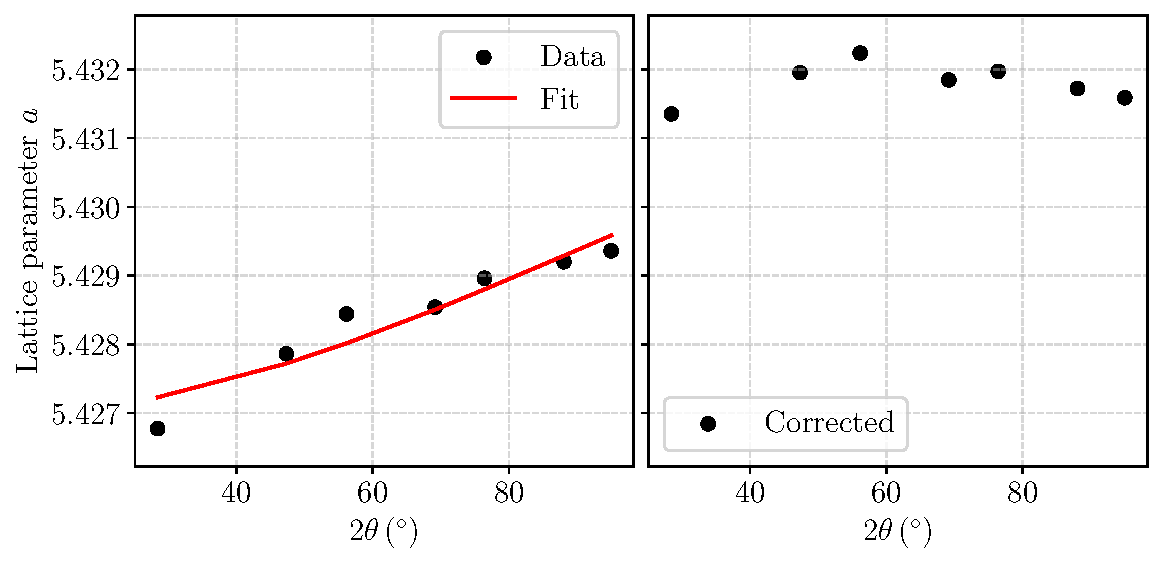
\includegraphics[width=\columnwidth]{analysis/offset_correction.pdf}
  \caption{Correction of the height offset in the polycrystalline silicon sample. The left panel shows the fit of \eq{\ref{eq:model}} to the data in \tab{\ref{tab:lattice-parameter}}. The right panel shows the corrected lattice parameters.}
  \label{fig:fit-poly}
\end{figure}

\subsection{Single-crystal silicon}

We also measured two samples of single-crystal silicon. Our goal was to identify the orientation of a ``standard'' cut and to confirm the lack of diffraction peaks from a sample cut along a non-symmetric direction.

For the first sample, the scan revealed a single peak, shown in \fig{\ref{fig:peaks-single-std}}. By comparing it to the pattern from polycrystalline silicon (\fig{\ref{fig:peaks-poly-b}}), we see that it aligns with the fourth peak, corresponding to the (400) plane, which indicates that the crystal was cut along this direction. The presence of a single sharp peak is consistent with the expectation for a well-aligned single crystal.

The second sample was labeled as a (510) cut. Since the (510) direction is not a symmetry direction of the silicon lattice \cite{Si}, we expect no diffraction peaks when the sample is aligned in this orientation. As shown in \fig{\ref{fig:peaks-single-510}}, the scan does not display any distinct peaks, only background scattering at low angles. This confirms that the crystal is indeed oriented along a non-symmetric direction.

\begin{figure}
  \centering
  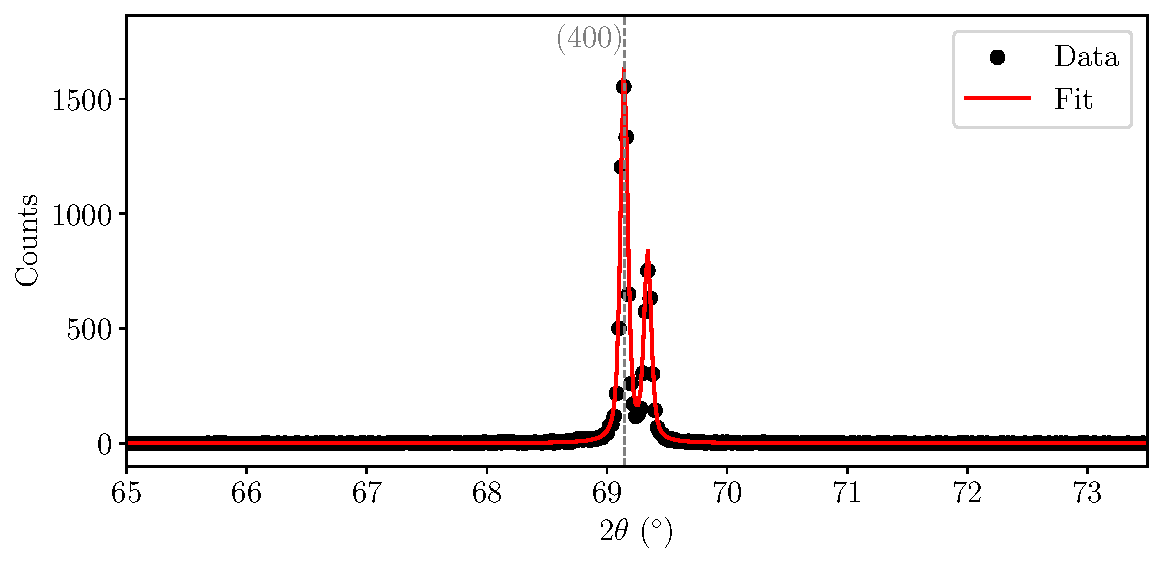
\includegraphics[width=\columnwidth]{analysis/peaks-Si_single_crystal-std.pdf}
  \caption{X-ray diffraction of single-crystal silicon in a ``standard'' cut.}
  \label{fig:peaks-single-std}
\end{figure}

\begin{figure}
  \centering
  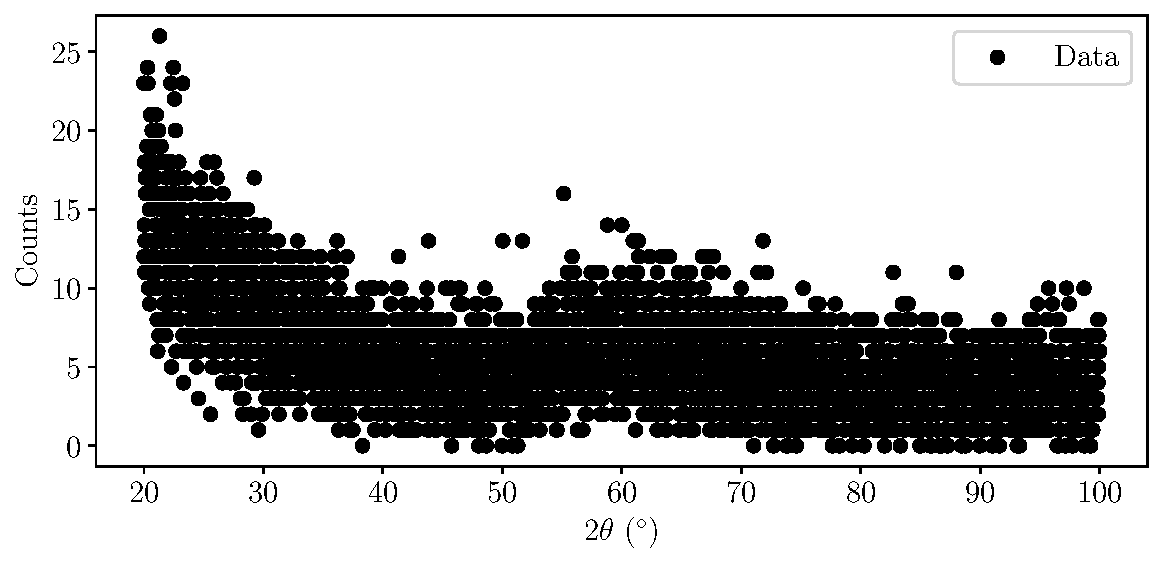
\includegraphics[width=\columnwidth]{analysis/peaks-Si_single_crystal-510.pdf}
  \caption{X-ray diffraction of single-crystal silicon in a (510) cut.}
  \label{fig:peaks-single-510}
\end{figure}

\subsection{Superconductor}

Finally, we collaborated with students from the Superconductivity lab to analyze two samples of YBa$_2$Cu$_3$O$_7$, a high-temperature ceramic-oxide superconductor \cite{Superconductivity}. The samples (labeled M3 and M4) were prepared with different annealing conditions during the second heating cycle. Sample M3 was sintered in flowing oxygen for 16 hours at $950^\circ$C, while sample M4 was heated to $950^\circ$C for 8 hours in air using the muffle furnace.

Our goal was to determine whether these differences in preparation led to detectable changes in crystal structure. The resulting diffraction patterns, shown in \fig{\ref{fig:peaks-super}}, reveal that the two samples exhibit nearly identical peaks. This suggests that the differing annealing atmospheres and durations did not significantly affect the crystal structure.

Additionally, all observed peaks match those expected for YBa$_2$Cu$_3$O$_7$ based on literature data \cite{YBa2Cu3O7}. This indicates that the samples are pure and that there is no significant presence of residual starting materials.

\begin{figure}
  \centering
  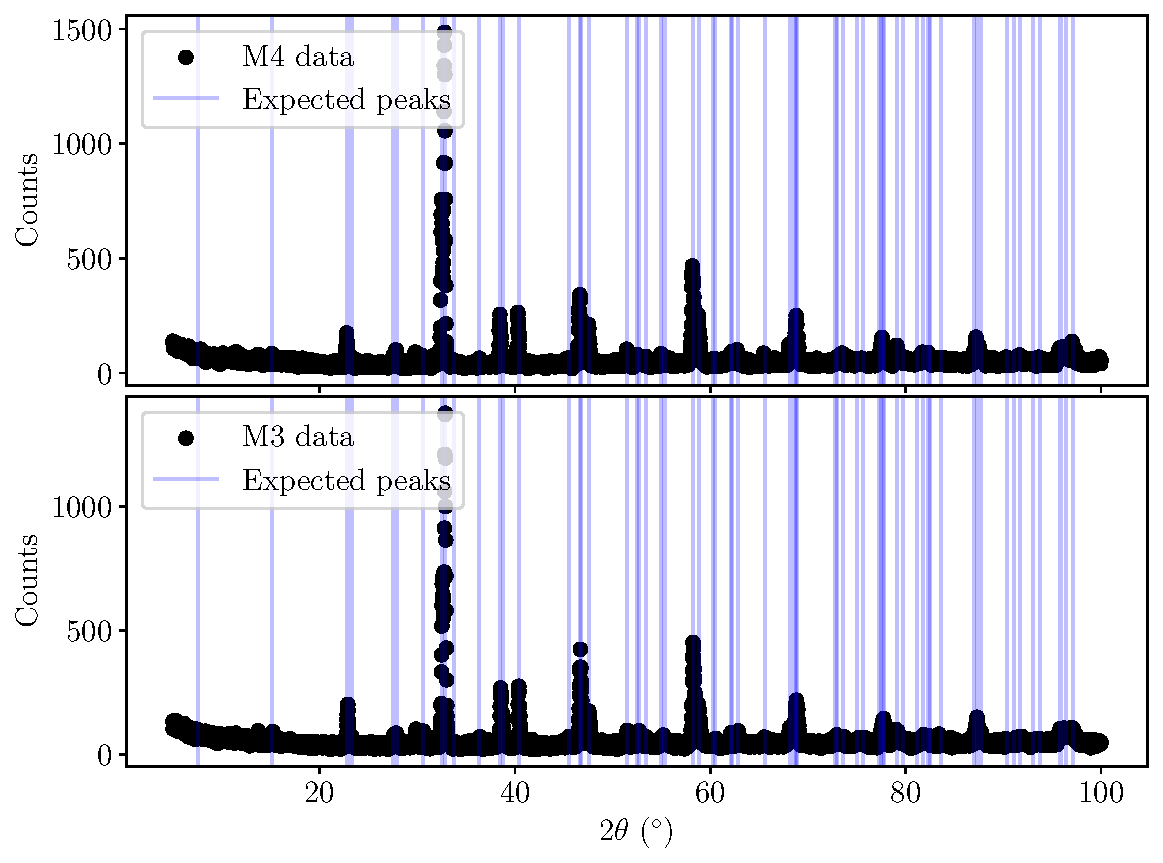
\includegraphics[width=\columnwidth]{analysis/peaks-YBa2Cu3O7.pdf}
  \caption{X-ray diffraction of two YBa$_2$Cu$_3$O$_7$ samples prepared under different conditions.}
  \label{fig:peaks-super}
\end{figure}

\section{Conclusion}\label{sec:conclusion}

In this experiment, we used X-ray diffraction to investigate the crystal structures of different materials. By analyzing a polycrystalline silicon sample, we determined its lattice parameter to be $a = 5.4318(3)$ \AA{} after correcting for a systematic offset. This result is in good agreement with the literature and demonstrates the sensitivity of diffraction measurements to sample alignment.

We also examined two single-crystal silicon samples to determine their orientation. By comparing their diffraction patterns to that of the polycrystalline sample, we identified one as a (400) cut, while the absence of peaks in the other confirmed its orientation along the non-symmetric (510) direction.

Finally, we compared two samples of the high-temperature superconductor YBa$_2$Cu$_3$O$_7$ prepared under different annealing conditions. The nearly identical diffraction patterns indicate that the differences in preparation did not lead to detectable structural changes. Moreover, the agreement with literature data indicates that both samples are pure.

These results highlight the importance of X-ray diffraction as a tool for characterizing crystal structures and detecting subtle differences in material preparation.

\begin{acknowledgements}
  This work was done in collaboration with Sage Weisrock under the supervision of Professor Yumi Ijiri. I thank students from the Superconductivity lab -- Anya Molodtsova, Avay Subedi, and John Duffy -- for providing the YBa$_2$Cu$_3$O$_7$ samples used in our measurements. I am especially grateful to Avay Subedi for sharing details about their preparation conditions.
\end{acknowledgements}

\bibliography{refs}

\end{document}
